\section{Resultados}



\subsection{probando con 50 elementos }

Estableciendo N=50 .






   

   .

   



\begin{figure}[H]
  \centering
  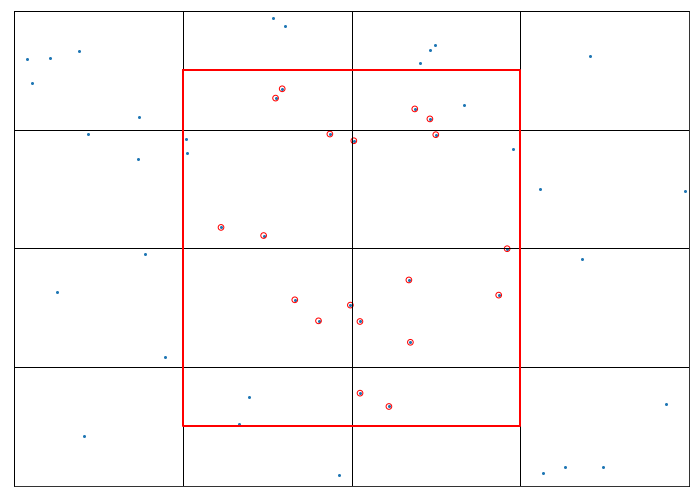
\includegraphics[width=0.8\textwidth]{imagenes/search-quadtree.png}
 % \label{fig:act-1}
\end{figure}


\begin{figure}[H]
  \centering
  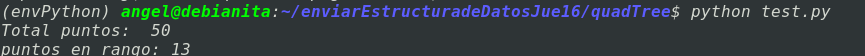
\includegraphics[width=1\textwidth]{imagenes/rango.png}
 % \label{fig:act-1}
\end{figure}

En la figura  el rango osea la cantidad de puntos  dentro del cuadrado rojo son 13 \cite{repo}.

\section{discusión}



 Quadtree no trabaja bien  cuando debe almacenar gran cantidad de diferentes píxeles existentes en una imagen con muchos colores, dado que podría tomar un tamaño excesivamente grande.
    También por ser una estructura de datos de memoria principal, al querer representar imágenes muy grandes, muchas veces el Quadtree no puede ser almacenado en dicha memoria. En esos caso, es mejor usar  estructuras alternativas por ejemplo, un B+ tree, para compensar esa limitación.


\section{conclusión}

Los Quadtrees son una forma de dividir el espacio para que sea fácil de intersecar y buscar.
La detección de colisiones puede ser una operación costosa y puede ralentizar el rendimiento  . Los Quadtrees son una forma en que puede ayudar a acelerar la detección de colisiones y mantener por ejemplo un juego funcionando a la máxima velocidad.
